\documentclass[10pt,a4paper,spanish]{report}

\usepackage[spanish]{babel}
\usepackage[utf8]{inputenc}
\usepackage{amsmath, amsthm}
\usepackage{amsfonts, amssymb, latexsym}
\usepackage{enumerate}
\usepackage[official]{eurosym}
\usepackage{graphicx}
\usepackage[usenames, dvipsnames]{color}
\usepackage{colortbl}
\usepackage{multirow}
\usepackage{fancyhdr}
\usepackage[all]{xy}
\usepackage{minted}
\usepackage{tikz}
\usepackage{pgfplots}
\usepackage{algpseudocode}
\usepackage{listings}
\usepackage{titlesec}

\pgfplotsset{compat=1.5}

% a4large.sty -- fill an A4 (210mm x 297mm) page
% Note: 1 inch = 25.4 mm = 72.27 pt
%       1 pt = 3.5 mm (approx)

% vertical page layout -- one inch margin top and bottom
\topmargin      0 mm    % top margin less 1 inch
\headheight     0 mm    % height of box containing the head
\headsep       10 mm    % space between the head and the body of the page
\textheight   250 mm
\footskip      14 mm    % distance from bottom of body to bottom of foot

% horizontal page layout -- one inch margin each side
%\oddsidemargin    0   mm    % inner margin less one inch on odd pages
%\evensidemargin   0   mm    % inner margin less one inch on even pages
%\textwidth      159.2 mm    % normal width of text on page

\usepackage[math]{iwona}
\usepackage[T1]{fontenc}
\usepackage{inconsolata}

\usepackage[pdftex, bookmarks=true,
	bookmarksnumbered=false, % true means bookmarks in
	% left window are numbered
	bookmarksopen=false,     % true means only level 1
	% are displayed.
	colorlinks=true,
linkcolor=webblue]{hyperref}

\definecolor{webgreen}{rgb}{0, 0.5, 0} % less intense green
\definecolor{webblue}{rgb}{0, 0, 0.5}  % less intense blue
\definecolor{webred}{rgb}{0.5, 0, 0}   % less intense red
\definecolor{dblackcolor}{rgb}{0.0,0.0,0.0}
\definecolor{dbluecolor}{rgb}{.01,.02,0.7}
\definecolor{dredcolor}{rgb}{0.8,0,0}
\definecolor{dgraycolor}{rgb}{0.30,0.3,0.30}

\newcommand{\HRule}{\rule{\linewidth}{0.5mm}} % regla horizontal para  el titulo

\pagestyle{fancy}
%con esto nos aseguramos de que las cabeceras de capítulo y de sección vayan en minúsculas

\renewcommand{\chaptermark}[1]{%
	\markboth{#1}{}}
\renewcommand{\sectionmark}[1]{%
	\markright{\thesection\ #1}}
\fancyhf{} %borra cabecera y pie actuales
\fancyhead[LE,RO]{\bfseries\thepage}
\fancyhead[LO]{\bfseries\leftmark}
\renewcommand{\headrulewidth}{0.5pt}
\renewcommand{\footrulewidth}{0pt}
\addtolength{\headheight}{0.5pt} %espacio para la raya
\fancypagestyle{plain}{%
	\fancyhead{} %elimina cabeceras en páginas "plain"
	\renewcommand{\headrulewidth}{0pt} %así como la raya
}

%%%%% Para cambiar el tipo de letra en el título de la sección %%%%%%%%%%%
\chapterfont{\fontfamily{pag}\selectfont} %% for chapter if you want
\sectionfont{\fontfamily{pag}\selectfont}
\subsectionfont{\fontfamily{pag}\selectfont}
\subsubsectionfont{\fontfamily{pag}\selectfont}
\titleformat{\chapter}{\normalfont\Huge}{}{0pt}{\Huge} % Capítulos sin "Capítulo x" encima del título

\renewcommand{\labelenumi}{\arabic{enumi}. }
\renewcommand{\labelenumii}{\labelenumi\alph{enumii}) }
\renewcommand{\labelenumiii}{\labelenumii\roman{enumiii}: }

\newmintedfile[myPascal]{pas}{
	linenos,
	numbersep=5pt,
	gobble=0,
	fontsize=\footnotesize
}

\newmintedfile[myLex]{bash}{
	linenos,
	numbersep=5pt,
	gobble=0,
	frame=lines,
	framesep=2mm,
	breaklines=true,
	fontsize=\footnotesize
}

\newmintedfile[myLatex]{tex}{
	linenos,
	numbersep=5pt,
	gobble=0,
	frame=lines,
	framesep=2mm,
	tabsize=3,
}

\newmintedfile[myHtml]{html}{
	linenos,
	numbersep=5pt,
	gobble=0,
	frame=lines,
	framesep=2mm,
	tabsize=3,
}

\title{Modelos de Computación}
\author{David Sánchez Jiménez}

\begin{document}
\begin{titlepage}
	\begin{center}
		\HRule \\[0.8cm]
		\textsc{\huge Informática\\[0.5cm] Industrial}\\[1.6cm]
		\HRule \\[1cm]
		\begin{flushleft}
			\emph{Hecho por:}\\
			David Sánchez Jiménez
		\end{flushleft}
		\vspace{12cm}
		\large{\today}\\
		\vspace{0.5cm}
		\htmladdnormallink{
\includegraphics[width=2cm]{88x31.png}}
		{http://creativecommons.org/licenses/by-nc/4.0/}\\[0.5cm]
		\texttt{Prácticas de Informática Industrial\\ by
			\href{mailto:dasaji92@gmail.com}{David Sánchez Jiménez} is licensed under a \htmladdnormallink{Creative Commons Reconocimiento-NoComercial-CompartirIgual 4.0 Internacional License}
			{http://creativecommons.org/licenses/by-nc/4.0/}}.\\[3mm]
	\end{center}
\end{titlepage}

\tableofcontents
\newpage

%%%%%%%%%%%% Práctica 1 %%%%%%%%%%%%
\chapter{Esquema de Simulación Intouch}

\noindent
En esta práctica vamos a realizar la simulación de dos tanques interconectados mediante una válvula para desaguar el tanque superior y una bomba para subir el agua del tanque inferior al tanque superior.

\begin{figure}[!hbp]
	\centering  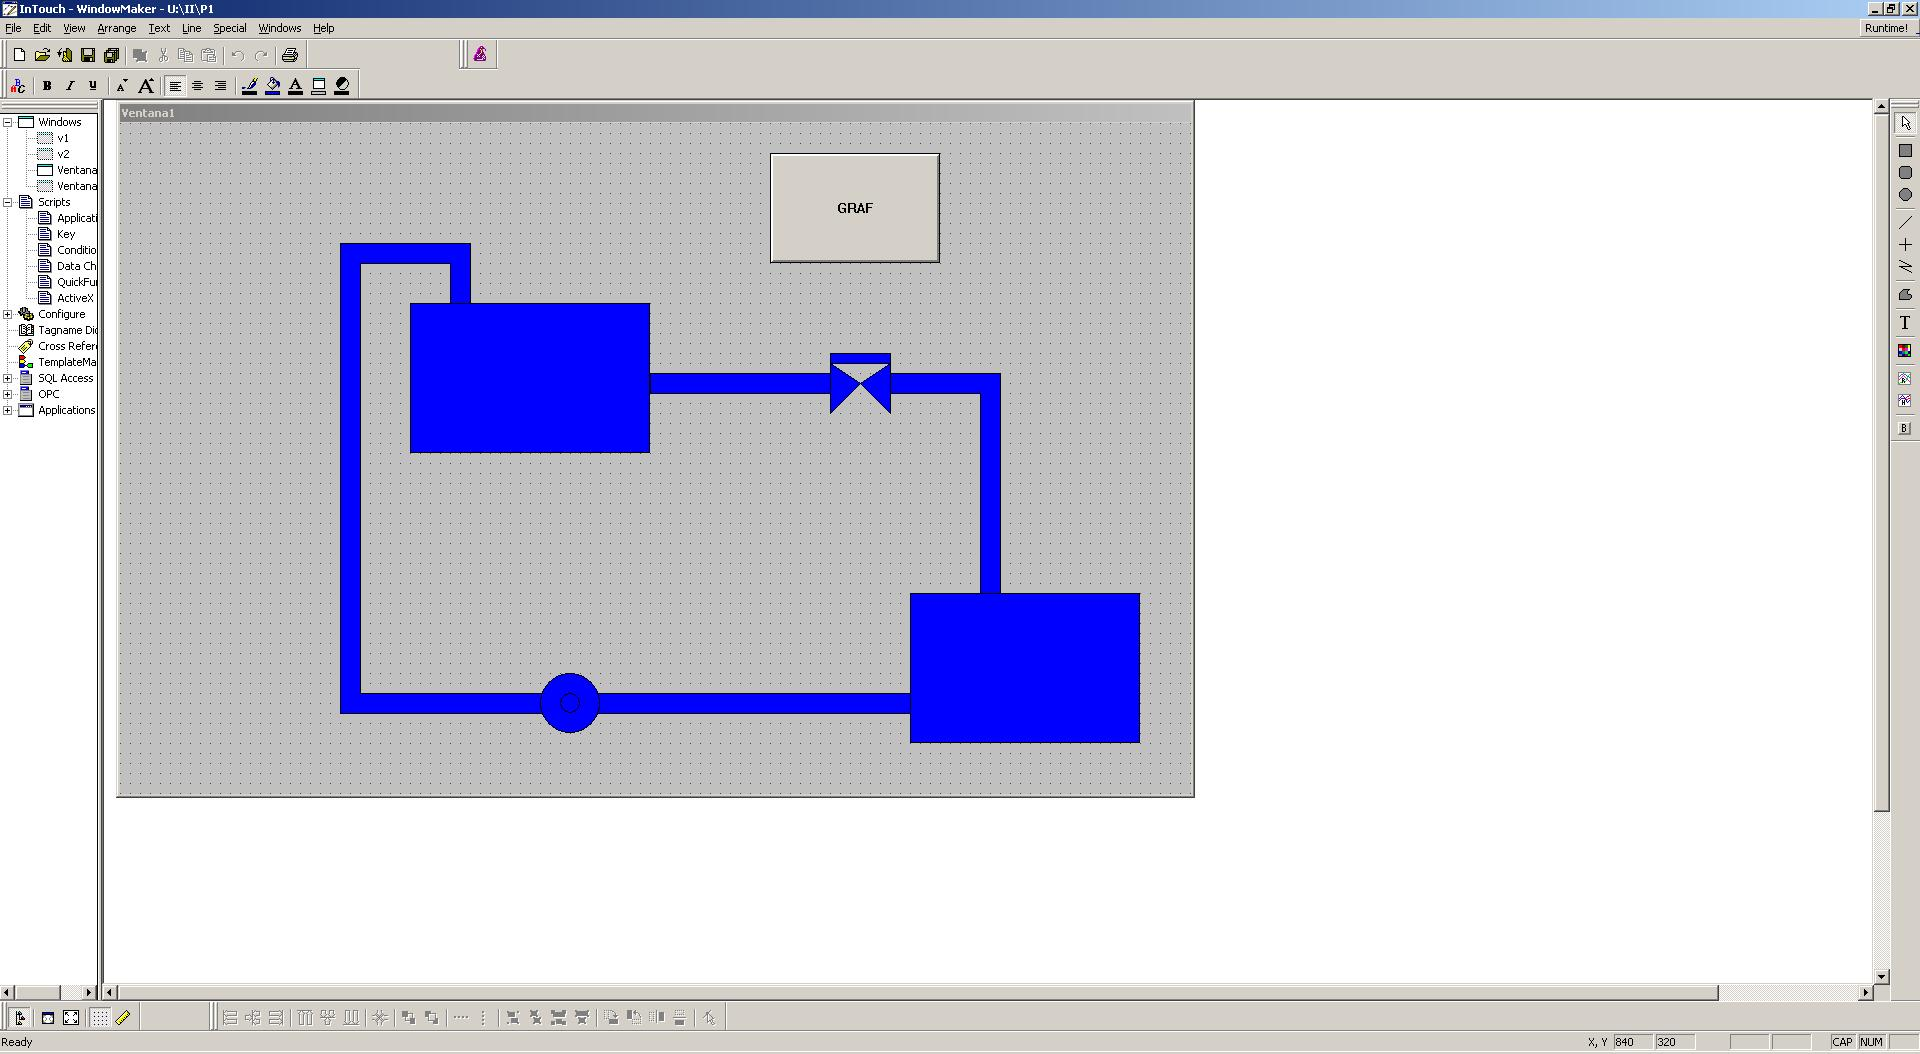
\includegraphics[width=0.9\textwidth]{Imagenes/p1.JPG}
\end{figure}

\noindent
El script utilizado es el siguiente:
\myPascal{Imagenes/P1.pas}

%%%%%%%%%%%% Práctica 2 %%%%%%%%%%%%
\chapter{Monitor de Control para SENSONYC}

\noindent
En esta practica vamos a realizar un un panel de control para la placa Sensonyc mediante el OPC de Intouch para controlar las distintas acciones que esta realiza mediante los distintos botones dispuestos. El panel de control desarrollado sería el siguiente:

\begin{figure}[!hbp]
	\centering  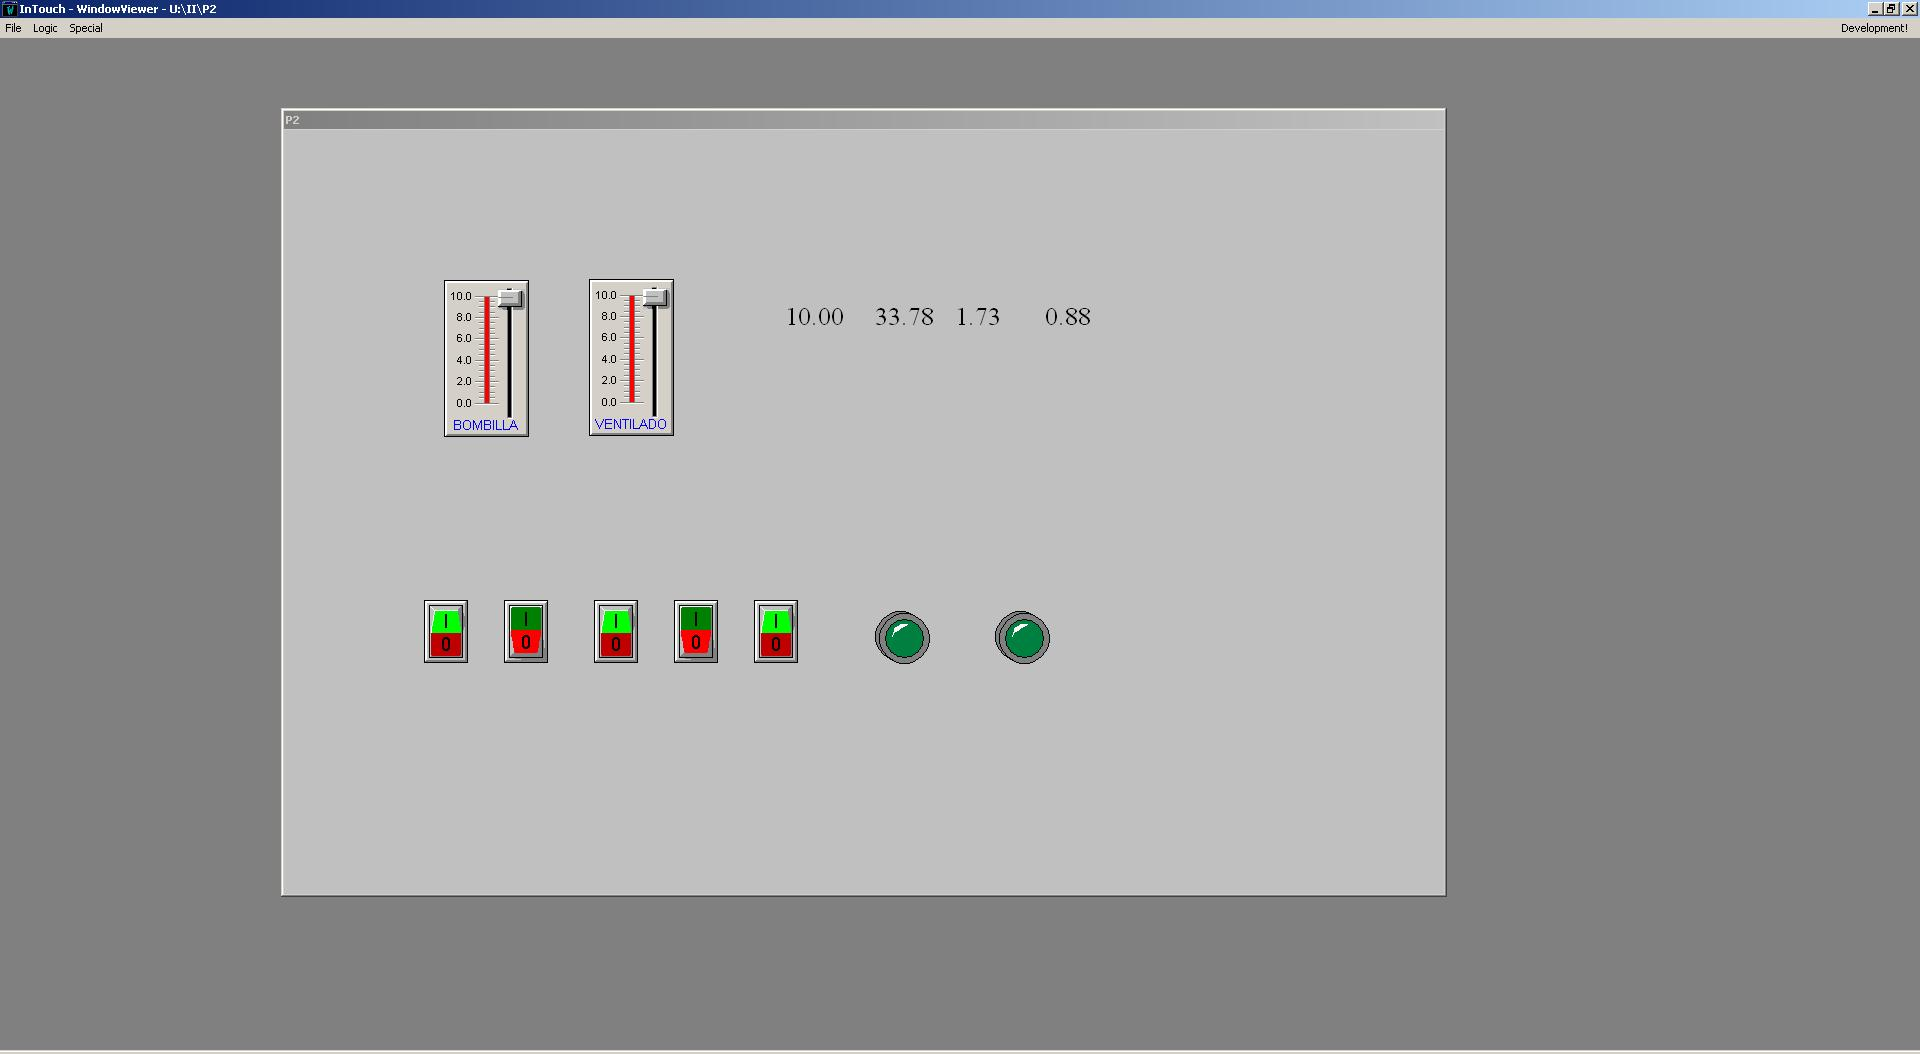
\includegraphics[width=1\textwidth]{Imagenes/p2.JPG}
\end{figure}

%%%%%%%%%%%% Práctica 3 %%%%%%%%%%%%
\chapter{Control Todo Nada de Temperatura}

\section{Control ON/OFF de temperatura}

\noindent
En esta práctica se gestionará la temperatura de una bombilla para que se encienda o se apague según el valor de consigna que le proporcionemos. Una vez se alcanza dicho valor de consigna la bombilla se apaga y se enciende el ventilador para enfriarla.

\begin{figure}[!hbp]
	\centering  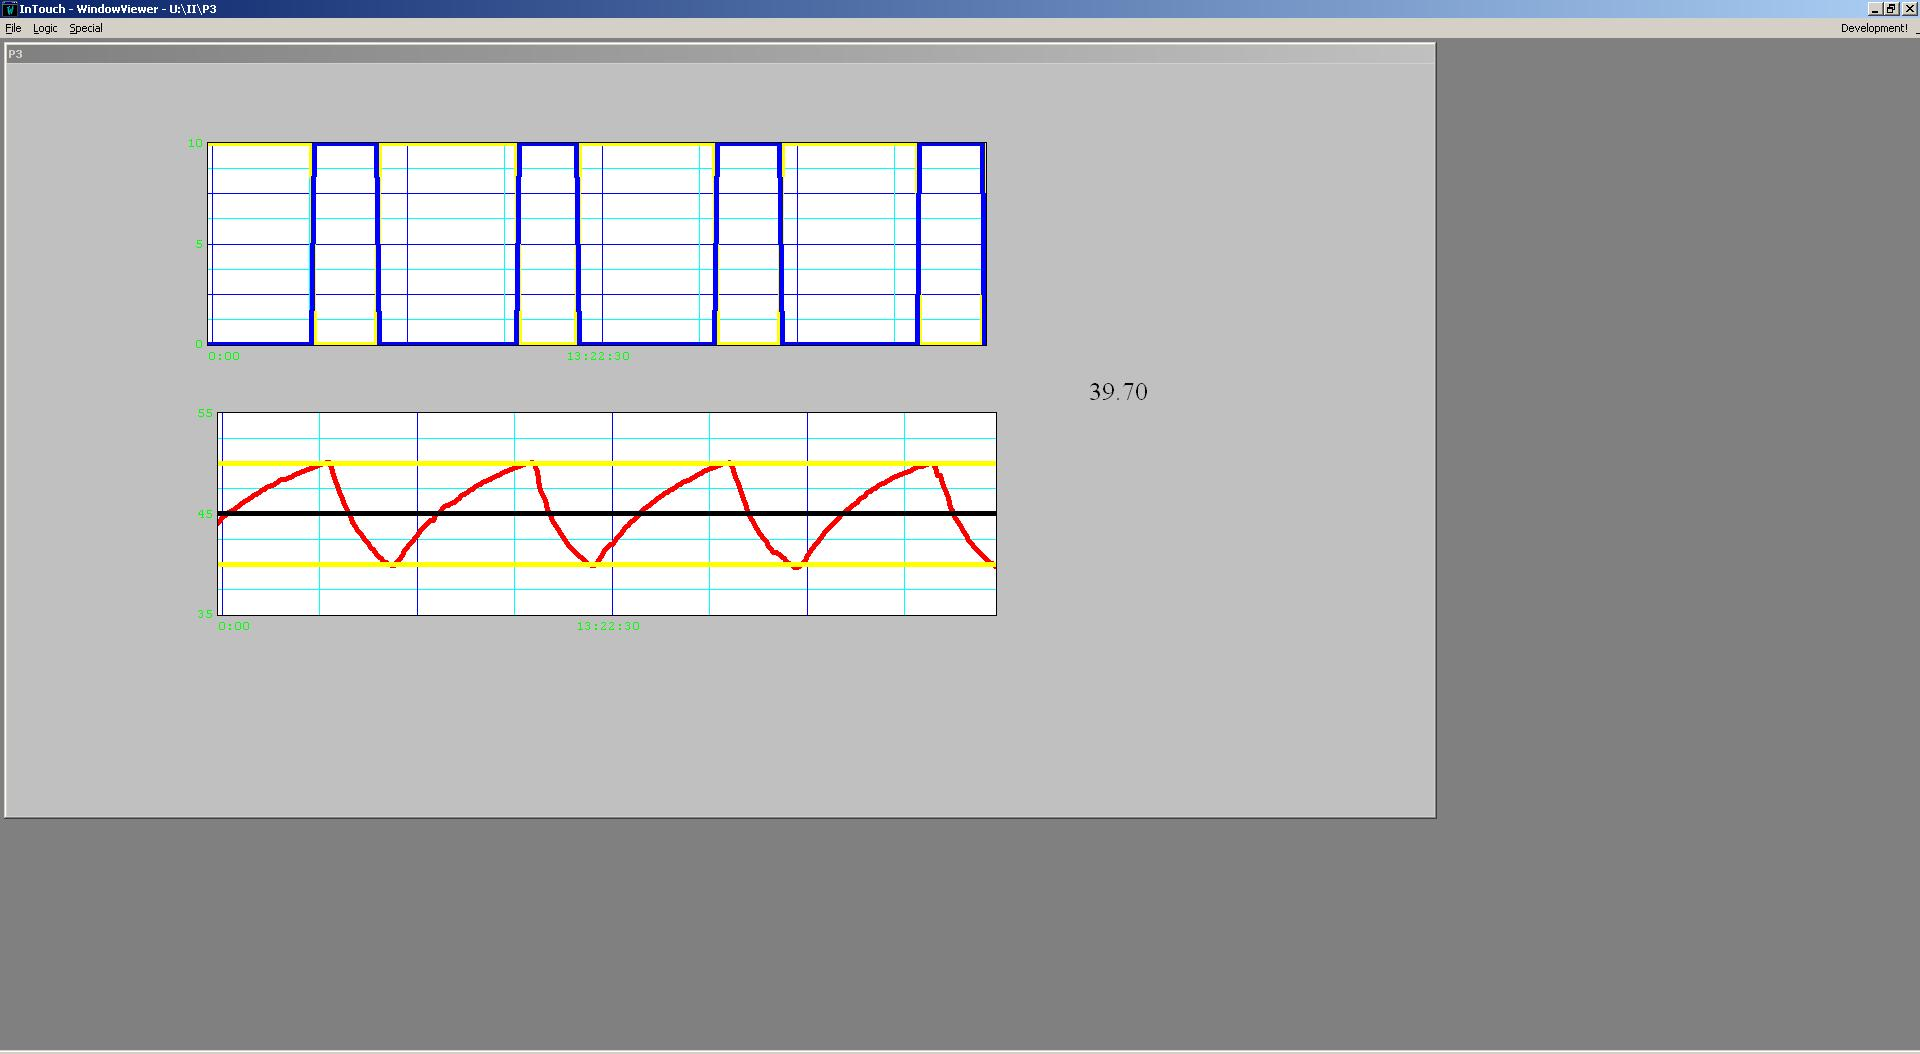
\includegraphics[width=1\textwidth]{Imagenes/p3-1.JPG}
\end{figure}

\noindent
El script utilizado es el siguiente:
\myPascal{Imagenes/P3-1.pas}

\newpage
\section{Control PID Discreto}

\noindent
En esta segunda parte vamos a refinar el funcionamiento de la práctica anterior para conseguir que la temperatura se estabilice al valor de consigna que le indiquemos.

\begin{figure}[!hbp]
	\centering  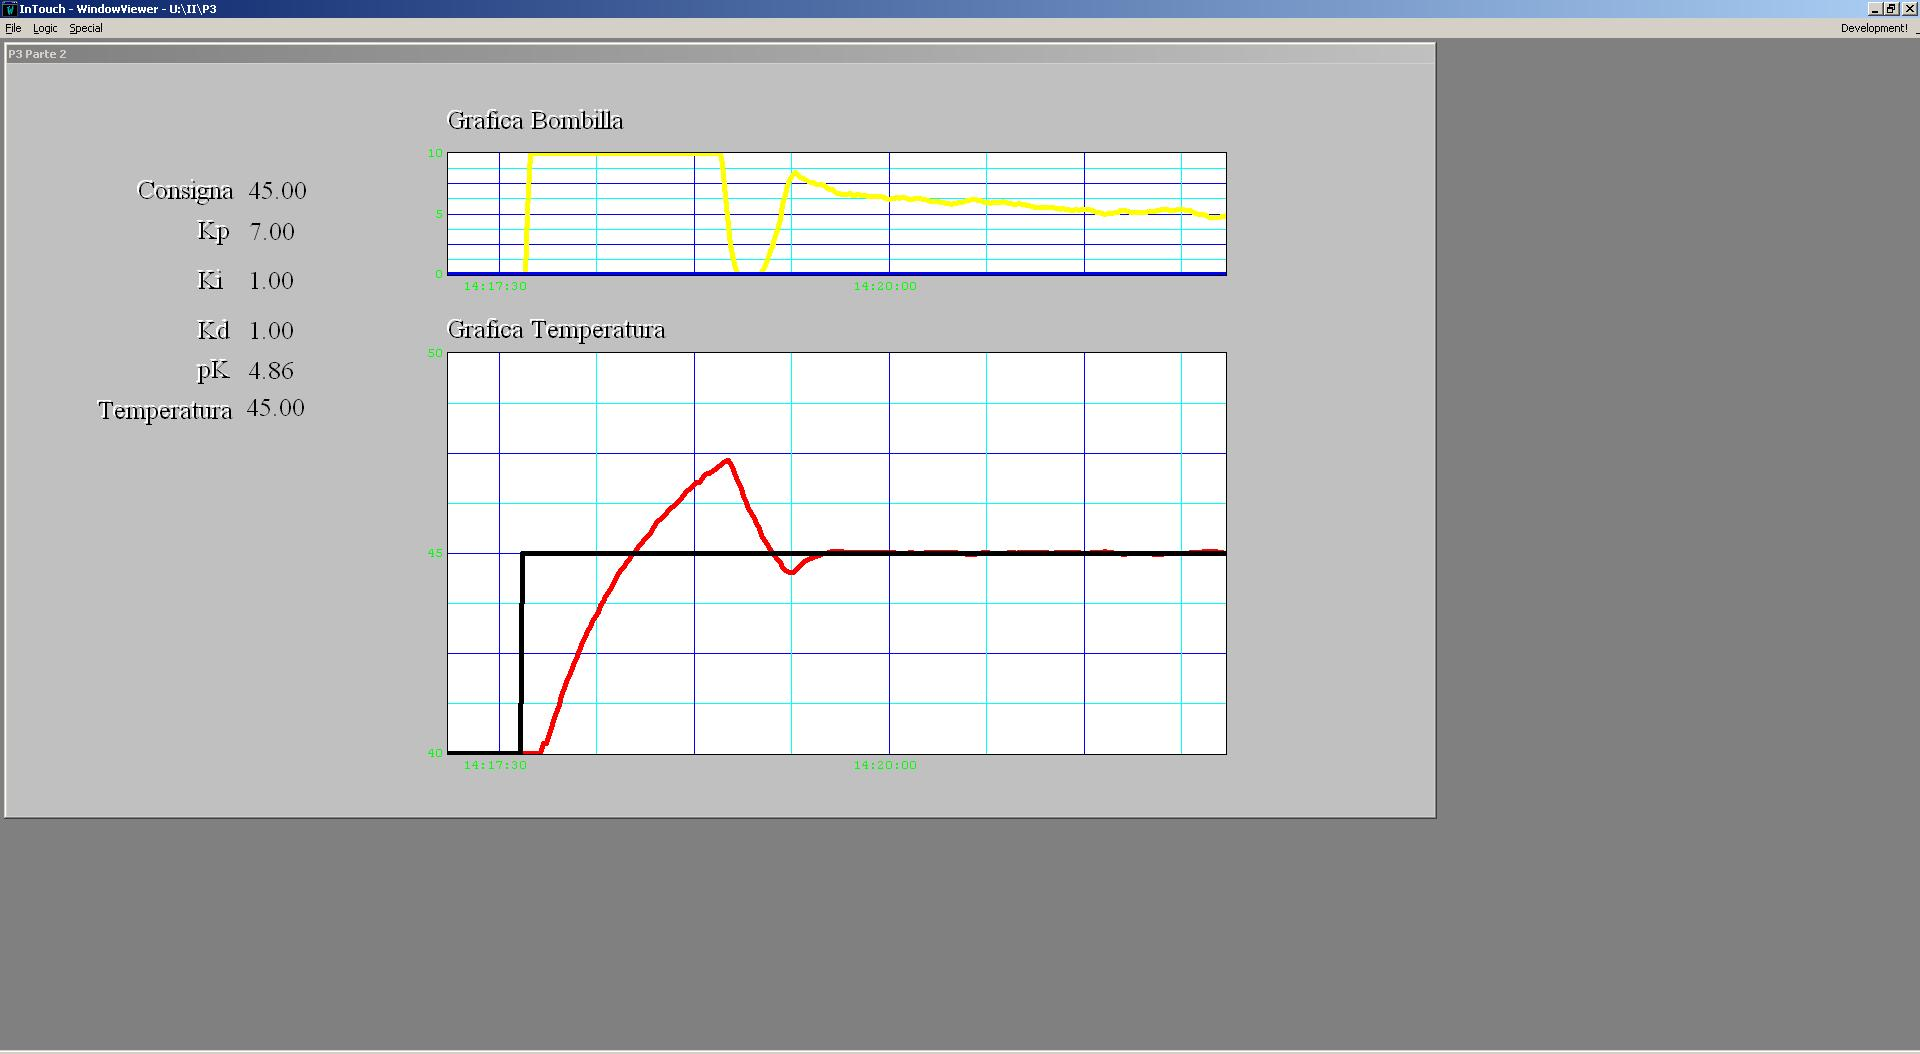
\includegraphics[width=1\textwidth]{Imagenes/p3-2.JPG}
\end{figure}

\noindent
El script utilizado sería el siguiente:
\myPascal{Imagenes/P3-2.pas}


%%%%%%%%%%%% Práctica 4 %%%%%%%%%%%%
\chapter{Control PID de Temperatura}

\noindent
En esta práctica vamos a realizar un ajuste experimental mediante método de ciclo límite para obtener los parámetros $K_P$, $K_I$ y $K_D$ con los algoritmos de Ziegler y Nichols y Aström y y Hägglund Hägglund. \\

\begin{figure}[!hbp]
	\centering  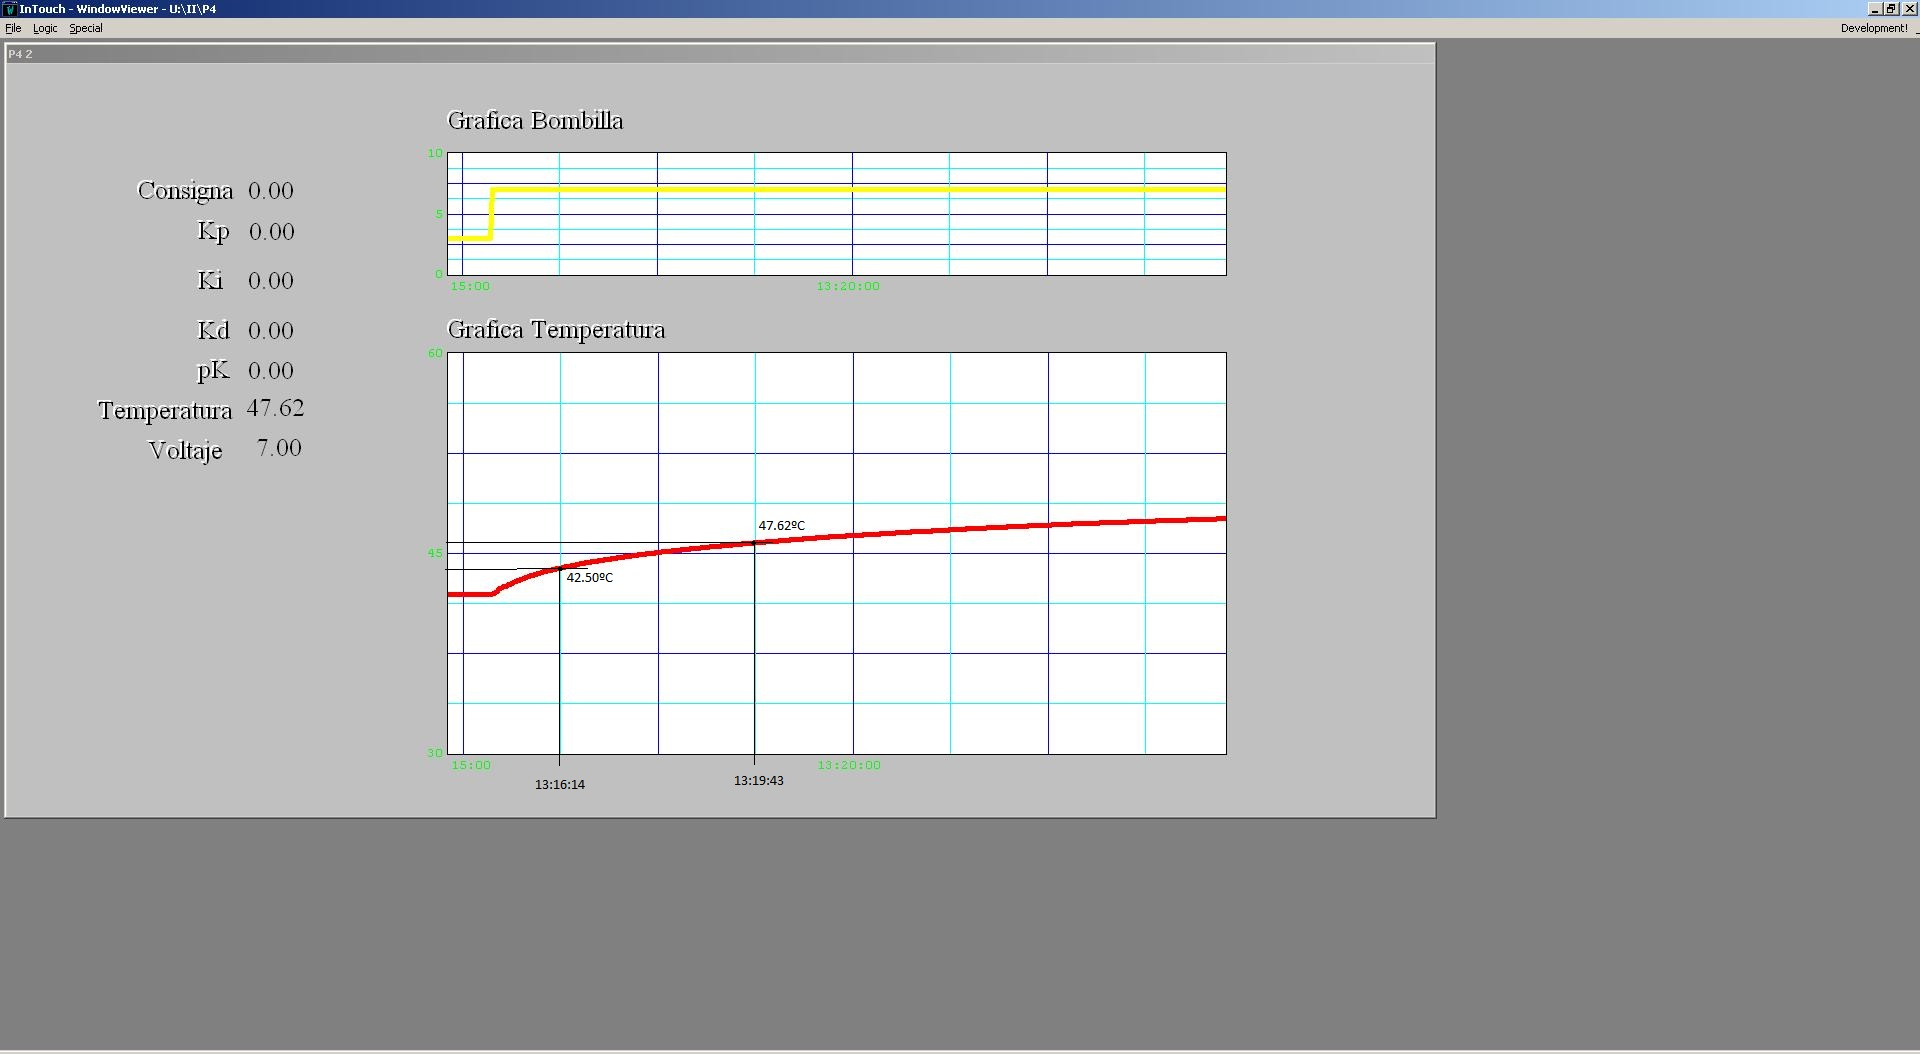
\includegraphics[width=1\textwidth]{Imagenes/p4.JPG}
\end{figure}

\noindent
Primero establecemos el voltaje de la bombilla a 3V y esperamos a que el valor de la temperatura obtenido en la gráfica se estabilice. En mi caso fué a 42.5ºC. A continuación provocamos un salto en el voltaje de bombilla y volvemos a esperar a que se estabilice la temperatura. Para realizar la captura de pantalla y que se aprecie el salto de voltaje provocado he considerado que la estabilización se realiza a 47.62ºC. \\

\noindent
Una vez tenemos registrados ambos valores de temperatura procedemos a realizar los calculos pertinentes.\\

\noindent
Primero obtenemos los valores de temperatura respectivos al $28.3\%$ y al $63.2\%$ y calculamos los tiempos $T_1$ y $T_2$ respectivamente.

\begin{displaymath}
	t_0 = 42.5 + 0.283 (47.62 - 42.5) = 43.948926^oC
\end{displaymath}
\begin{displaymath}
	t_1 = 42.5 + 0.632 (47.62 - 42.5) = 45.73584^oC
\end{displaymath}

\noindent
A continuación obtenemos el valor de K como el cociente entre cambios de temperatura y los valores de $T_p$ y $T_0$:

\begin{displaymath}
	K = \frac{T_1 - T_0}{V_1 - V_0} = \frac{47.62 - 42.50}{7 - 3} = 1.28
\end{displaymath}
\begin{displaymath}
	T_P = 1.5(t_2-t_1)=1.5(45.73584-43.948926)=2.680371
\end{displaymath}
\begin{displaymath}
	T_0 = 10-(t_2-T_p)=10(45.73584-2.680371)=-33.055469
\end{displaymath}

\noindent
Ahora podemos calcular $K_P$, $K_I$ y $K_D$:

\begin{displaymath}
	K_P = 1.2 \frac{T_p}{KT_0} = 1.2 \frac{2.680371}{1.28 x -33.055469} = −0.06334927
\end{displaymath}
\begin{displaymath}
	K_I = \frac{1}{2T_0} = \frac{1}{2 x -33.055469} = −0.01512609
\end{displaymath}
\begin{displaymath}
	K_D = 0.5 x T_0 = 0.5 x -33.055469 = −16.5277345
\end{displaymath}

%%%%%%%%%%%% Práctica 5 %%%%%%%%%%%%
\chapter{Control del Servomotor - Placas Fotovoltáicas}

\noindent
Con esta practica queremos controlar la posición del servomotor de manera que se posicione de forma que incida la máxima intensidad de luz sobre los dos paneles fotovoltaicos.

\begin{figure}[!hbp]
	\centering  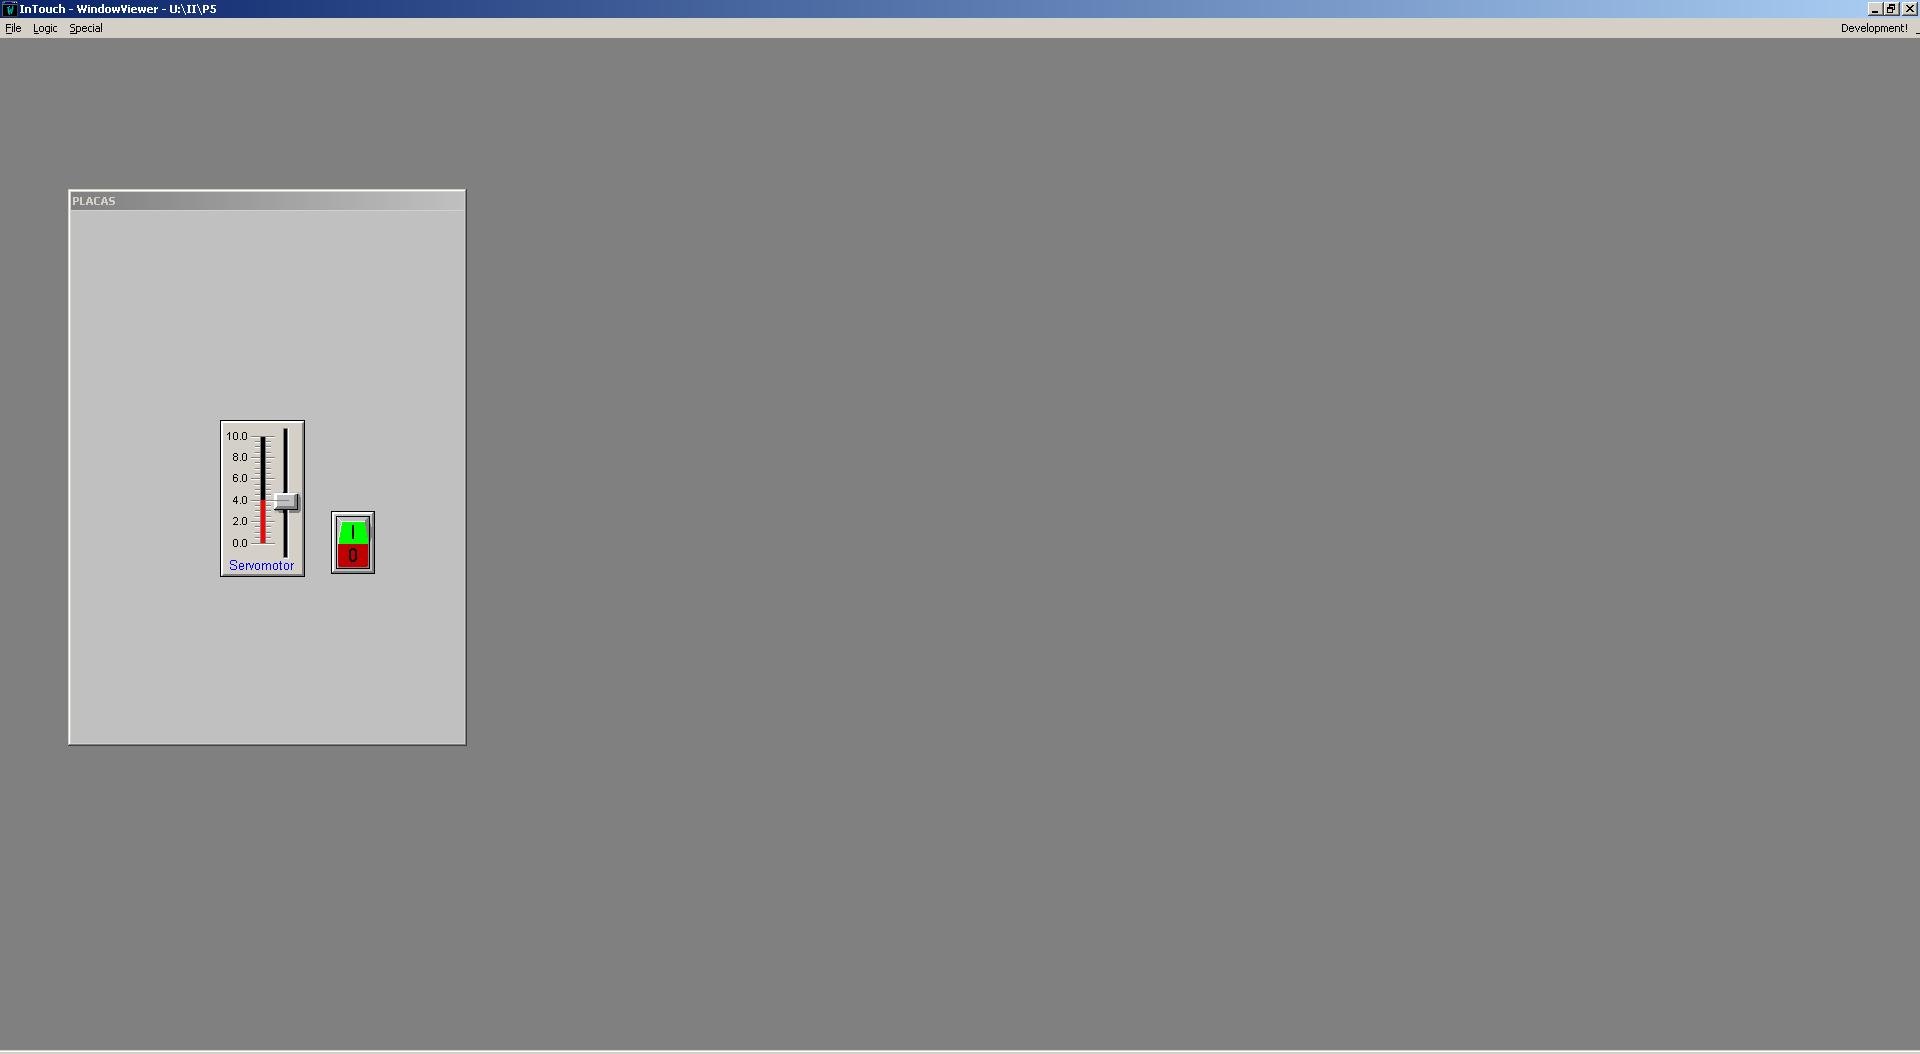
\includegraphics[width=1\textwidth]{Imagenes/p5.JPG}
\end{figure}

\noindent
El script utilizado sería el siguiente:
\myPascal{Imagenes/P5.pas}


\noindent
Un video del funcionamiento sería el siguiente:\\

\noindent
\href{https://drive.google.com/open?id=0BxFwsg5ejZuOdkRfZ3JWZzVfNmc}{https://drive.google.com/open?id=0BxFwsg5ejZuOdkRfZ3JWZzVfNmc}


\end{document}
